\chapter{Podsumowanie}
\section{Problemy konstrukcyjne i implementacyjne}
\label{cha:problems}
Największe dwa problemy z powstałą platformą to:
\begin{enumerate}
    \item Drukowana obudowa. - Konstrukcja taka pozostawia wiele do życzenia. Olbrzymie luzy na orczykach i ogólna giętkość wydrukowanych ekementów powoduje, że nie da się jednoznacznie ustalic parametrów kroku wystarczających do "zwyczajnego" przestawienia nogi. Trzeba brać znaczną poprawkę na giętkość konstrukcji, np. poprzez znacznie wyższy krok niż byłoby to faktycznie potrzebne.\\
    \item Platfotma o małej mocy obliczeniowej i węzeł napisany w Pythonie. - Niestety okazuje się że węzeł napisany w Pythonie nie jest w stanie nadążyć za węzłami napisanymi w \texttt{c++} i nie jest w stanie przetworzyć ramek tak szybko jak pozostałe węzły je wysyłają. 
\end{enumerate}

W tym miejscu warto także wspomnieć że przybliżona kinematyka odwrotna okazała się jak najbardziej wystarczająca, przy tak drobnych krokach nie wprowadziła istotnego błędu w ruchy robota.\\

\section{Przeprowadzone eksperymenty}
Platforma została stworzona w taki sposób, aby dało się przeprowadzić każdy możliwy eksperyment. Jednakże w ramach tej pracy skupiono się tylko na podstawowych testach.

\subsection{Zmiany czasówek}
Kod programu zawiera trzy czasówki które można modyfikować i w ramach eksperymentów podjęto próbę jak największego zmniejszenia tych wartości.\\

Pierwsza wartość to okres odpytywania sterownika Polulu Maestro o obecne pozycje serw i wysyłania sprzężenia zwrtonego z tymi informacjami. Ostatecznie udało się zejść do wartości $XX ms$. Inaczej mówiąc, jest to czas co jaki wywoływana jest funkcja \texttt{ros\_publisher\_timer\_callback} z klasy \texttt{MaestroRosWrapper} (rys. \ref{UML_maestro}).\\

Druga wartość to czas, co jaki jest wysyłana jest ramka z kolejnymi ruchami serwa pojedynczej nogi. Czas ten jest bezpośrednio związany z ilością ramek jakie węzeł Pythonowy jest w stanie przetworzyć w jdnostce czasu. Ostatecznie udało się zejść do wartości $XX ms$. Wspomniane wcześniej ramki są wysyłane z poziomu funkcji \texttt{RobotLegRos::publish\_servo\_position} (rys. \ref{UML_leg}).\\

Trecia wartość to czas, co ile algorytm próbuje wykonać kolejne kroki. Wartość ta jest bezpośrednio związana z dwoma poprzednimi czasówkami. Im bardziej zmniejszymy powyższe okresy, tym bardziej możemy przyspieszyć sam algorytm chodu. Jeżeli natomiast kolejne kroki algorytmu zostaną zbyt przyspieszone bez przyspieszania wartości leżących "pod spodem" algorytmu to robot będzie wykonywał bliżej nieokreślone ruchy, bez podnoszenia nogi nad ziemię. Ruch ten wygląda jakby u źródła problemu leżało zatrzymywanie się kroku i przechodzenie do kolejnego etapu algorytmu zanim krok zostanie w pełni wykonany. Może to być wywołane wieloma różnymi elementami i niestety przyczyna nie została dokładnie zweryfikowana. Jednakże jako że zmniejszanie dwóch powyższych czasówek powoduje że problem pojawia się przy coraz to szybszym algorytmie, to najprawdopodobniej winowającą jest brak aktualnego sprzężenia zwrotnego lub nieopublikowane wartości skolejkowane gdzieś w środku algorytmu. Ostatecznie udało się zminimalizować ten czas do XX. Inaczej mówiąc, jest to okres wywoałnia funkcji \texttt{ThreeLegsController::timer\_callback} (rys. \ref{UML_controller_generator}).\\

\subsection{Długość i wysokość kroku}
Po ustaleniu najszybszych możliwych ruchów dla tej platformy przeprowadzono eksperymenty z długością i wysokością kroku.\\

Początkowe wartości zostaly przyjęte intuicyjnie. Długość wynosiła $100 mm$ a wysokość $50 mm$. Jednakże tylna noga nie była w stanie osiągnąć takiej pozycji (końcówka nogi musiałaby znajdować się zbyt blisko środkowego serwa), dlatego długość ta została zmniejszona do $70mm$. Z wysokością także był problem, ponieważ z powodu gięcia się całej konstrukcji, trzeba było wysokość podnieść do $75mm$. Przy wartościach tych robot był w stanie wykonać krok. Co prawda każdorazowo uderzał podwoziem o ziemię, ale przemieszczał się do przodu. Z powodu gnącej się konstrukcji także wszelakie próby matematycznego obliczania takich parametrów kroku, aby robot wyrobił się z odstawieniem nogi zanim podwozie uderzy o ziemię zakończyły się niepowodzeniem. Została tylko opcja empirycznego dochodzenia do najlepszych wartości.\\

Pomimo liczych prób jednakże nie udało się znaleźć takich parametrów kroku, aby robot dał radę zrobić "czysty" krok, bez zaczepiania o ziemię. Ostatecznie ustalono wartości na $step_l = XXmm$ i $step_h = XXmm$, ponieważ przy takich wartościach krok wydawał się wyglądać najlepiej - czas styku nogi z podłożem był minimalny.

\section{Wnioski}
W ramach pracy udało się zrealizować z mniejszym lub większym sukcesem w zasadzie wszystkie założone punkty. Jako że robot faktycznie przemieszcza się do prozdu, można by powiedzieć że projekt zakończył się sukcesem, jednak ostatecznej konstrukcji (przedstawionej na zdj. \ref{img:final_photo}) która w ramach tej pracy powstała nie można uznać za udany produkt. Jest to raczej pierwszy prototyp na długiej drodze rozwoju tego projektu. Jest to jednak pierwszy prototyp który jak na pierwsze prototypy działa bardzo dobrze i spełnia swoją rolę idealnie - dokładnie pokazuje występujące problemy, możliwe sposoby ich naprawienia i potencjalne ścieżki rozwoju projektu.

\begin{figure}[h!]
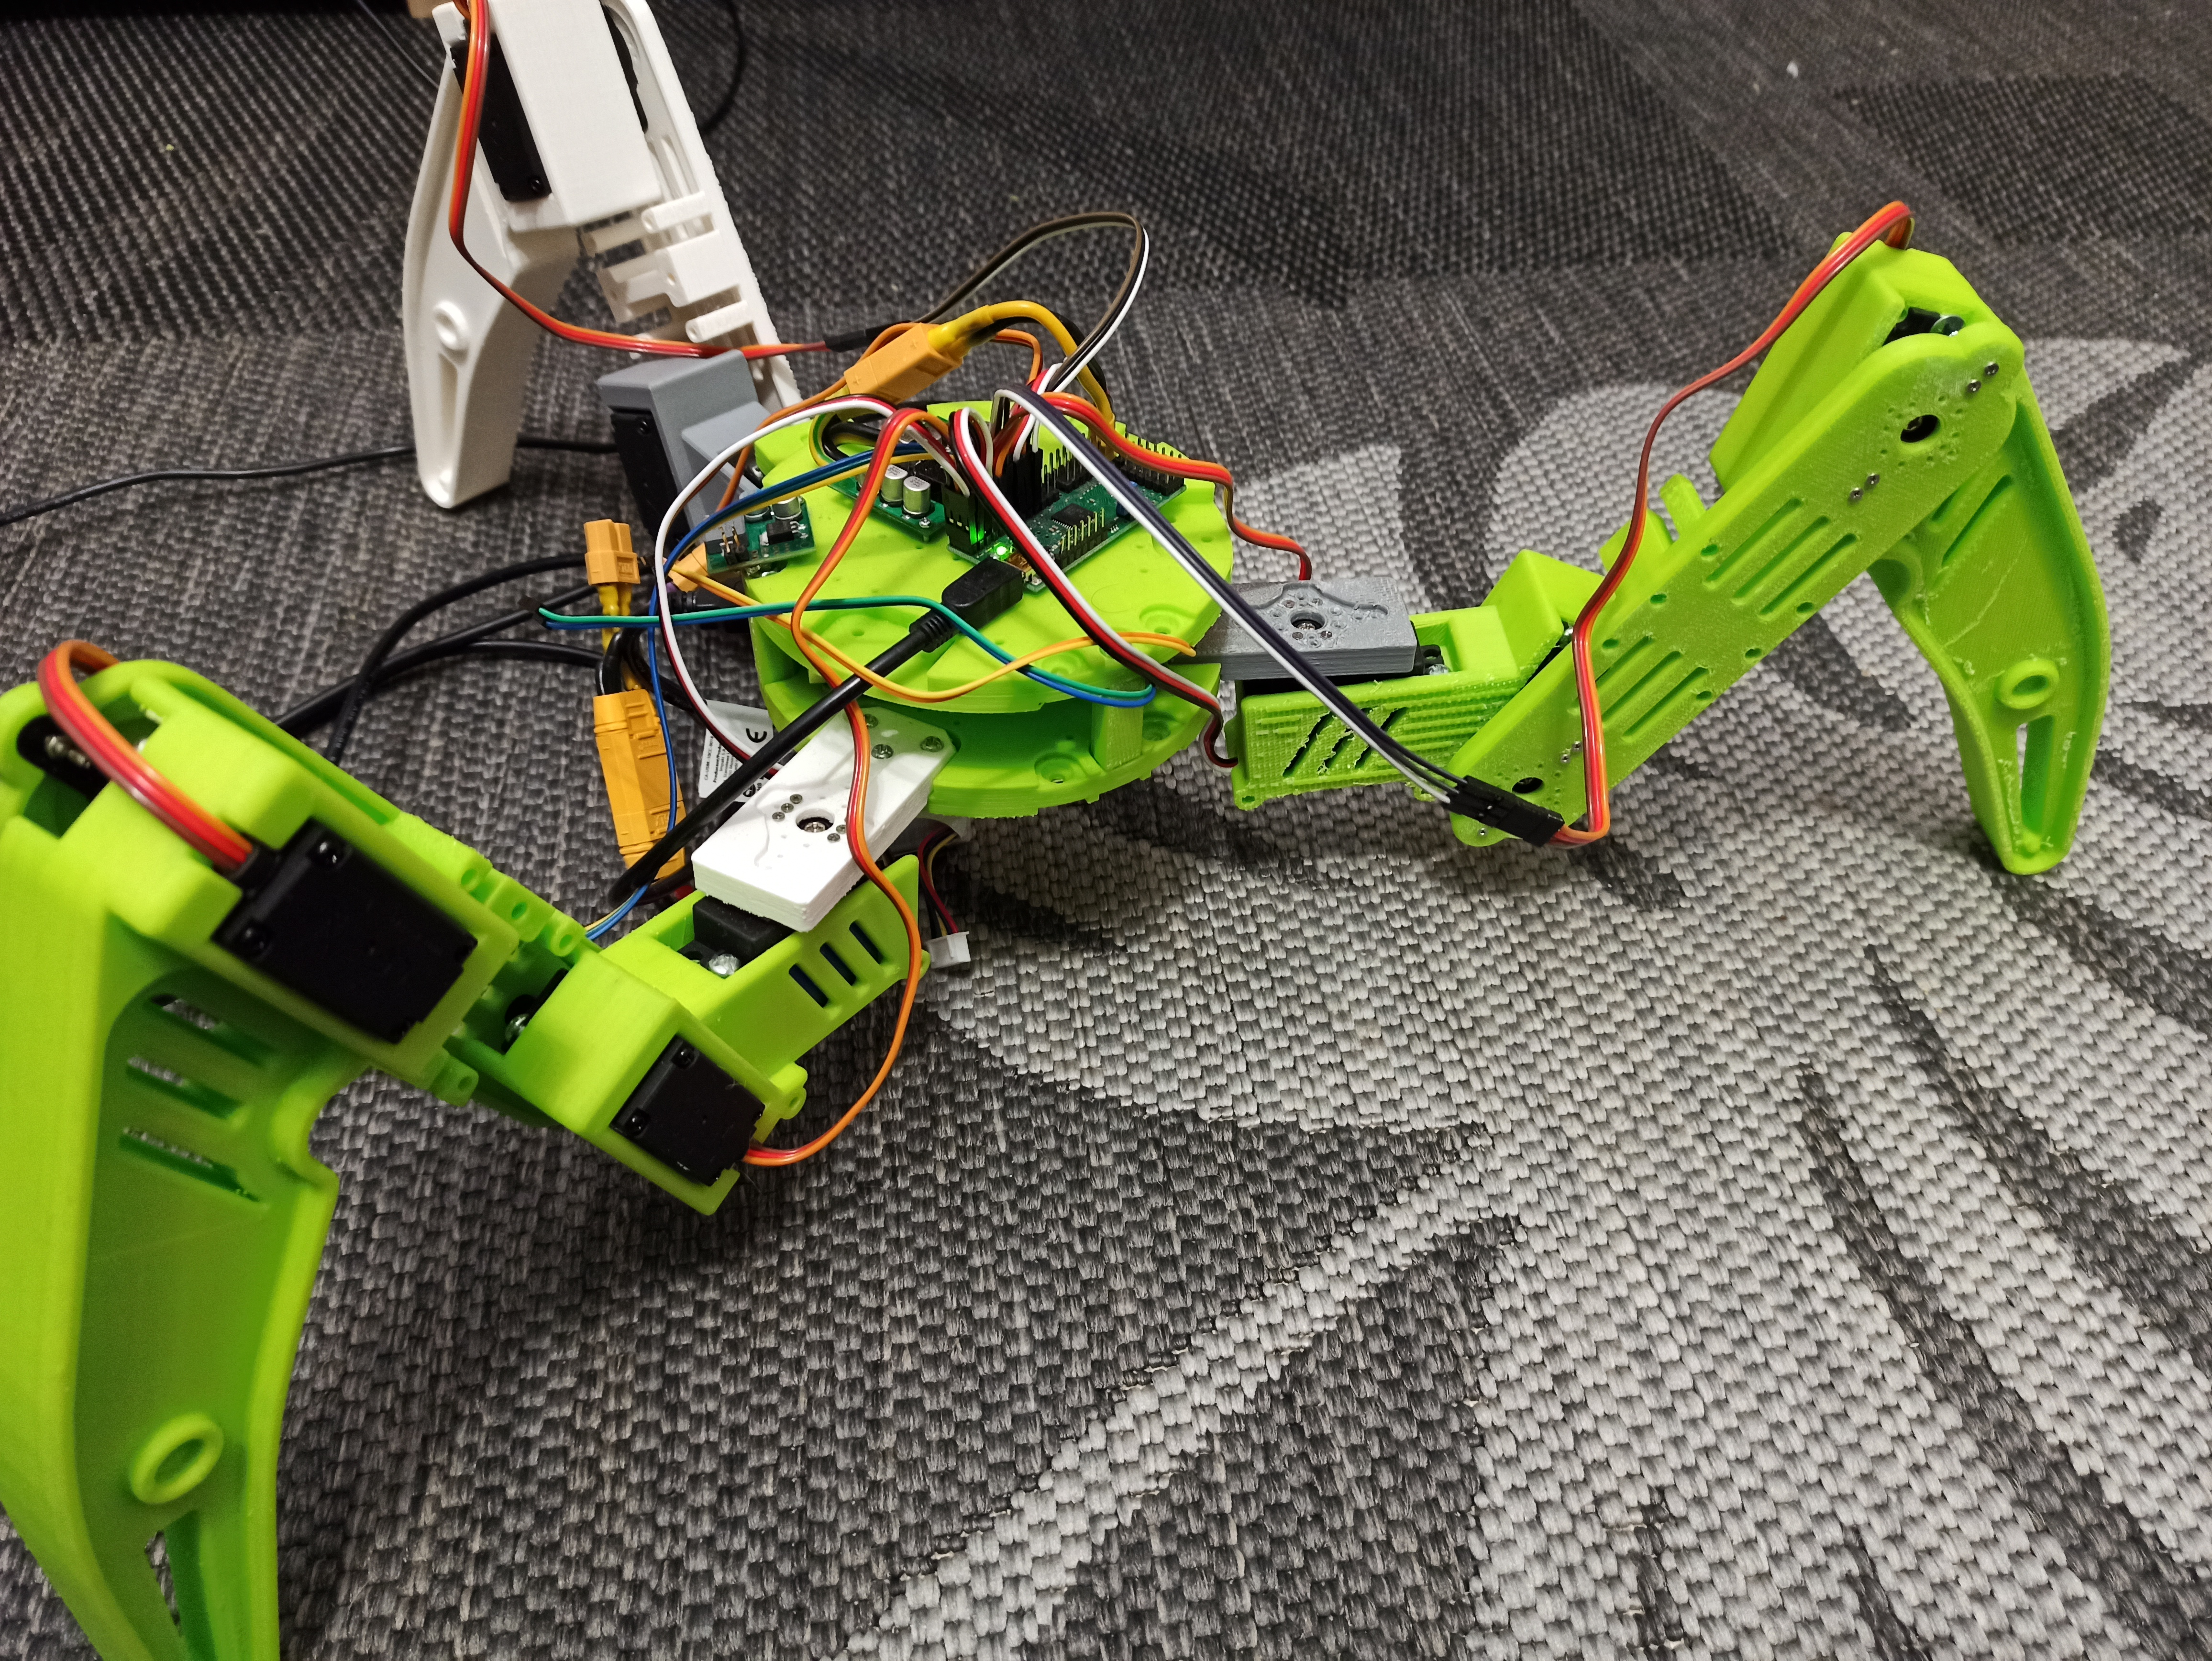
\includegraphics[width=0.7\textwidth]{img/final_photo.jpg}
\centering
\caption{Zdjęcie konstrukcji powstałej w ramach pracy.}
\label{img:final_photo}
\end{figure}

\section{Przyszły rozwój projektu}
Pierwszym krokiem rozwojowym powinno być naprawienie problemów wymienionych w podrozdziale \ref{cha:problems}. W pierwszej kolejności należałoby poprawić konstrukcję robota, dodając po przeciwnej stronie od każdego serwa na jego osi obrotu dodatkowy element usztywniający. Zapobiegłoby to gnięciu się elementów i luzom na serwach. Kolejną poprawką oczywiście byłoby przepisanie sterownika do serw do języka \texttt{c++}. Dałoby to drugą wersję prototypu, która byłaby już w pełni przygotowana do właśniwego rozwoju.\\

W ramach trzeciej wersji można by już postarać się przede wszystkim o dodanie węzła sterującego całą konstrukcją z poziomu gamepada i stworzenie dedykowanej płytki pcb aby dało się wygodnie powpinać w nią wszelakie komponenty. Dalej możliwości są nieskończone - można zrobić wszystko od eksperymentów z nogami o innej długości aż po montowanie lidarów i wszelakich innych systemów wizyjnych, sterujących platformą.
